%% ======================================================================
%% 04c_coupling_control.tex -- 3. Modelo (parte 4): controladores, modelo acoplado, propagacion
%% de perturbaciones y limitaciones fundamentales
%% ======================================================================
\subsection{Controladores y análisis en lazo cerrado}
\label{sec:control}

La Fig.~\ref{fig:loops} muestra los tres lazos y los acoplamientos físicos entre ellos. Cada lazo corre en su propio procesador y solo ve a los demás a través de la mecánica.

\begin{figure}[!htbp]
\centering
\begin{tikzpicture}[font=\footnotesize, >=Latex,
  blk/.style={draw, rounded corners=2pt, align=center, minimum height=10mm, inner xsep=3pt, inner ysep=2.5pt, line width=0.6pt, fill=#1},
  blk/.default=white]
  % lazo de la base (x: 0.00..5.62)
  \node[blk=pAzul!10, draw=pAzul, text width=2.48cm] (bc) at (1.35, 0.00) {myRIO\\ PI por rueda\\ + ir a un punto};
  \node[blk=pAzul!10, draw=pAzul, text width=1.88cm] (bp) at (4.62, 0.00) {base\\ \eqref{eq:basev}--\eqref{eq:motor}};
  \draw[->, line width=0.7pt] (bc) -- node[above=1.5pt]{$u_{R,L}$} (bp);
  \draw[->, line width=0.7pt] (bp.south) -- ++(0,-0.65) -| node[pos=0.25, below=1.5pt]{encoders, odometría \eqref{eq:odo}} (bc.south);

  % lazo del dron
  \node[blk=pVerde!10, draw=pVerde, text width=2.48cm] (dc) at (1.35, 3.15) {ESP32\\ P-I-D de ángulo $\to$\\ PI de velocidad\\ $\to$ \eqref{eq:alloc_inv}};
  \node[blk=pVerde!10, draw=pVerde, text width=1.88cm] (dp) at (4.62, 3.15) {octocóptero\\ en la rótula\\ \eqref{eq:pitchlin}};
  \draw[->, line width=0.7pt] (dc) -- node[above=1.5pt]{$\vect F$} (dp);
  \draw[->, line width=0.7pt] (dp.north) -- ++(0,0.72) -| node[pos=0.25, above=1.5pt]{IMU (filtro compl.)} (dc.north);

  % lazo de la bola (x: 9.05..13.70)
  \node[blk=pOcre!12, draw=pOcre, text width=1.98cm] (cc) at (10.12, 3.15) {ESP32-S3\\ PID sobre\\ $(x_b,y_b)$};
  \node[blk=pOcre!12, draw=pOcre, text width=1.98cm] (bb) at (10.12, 0.00) {bola en el\\ plato \eqref{eq:balllinx}};
  \node[blk=pGris!10, draw=pGris, text width=2.02cm] (cam) at (12.50, 1.58) {cámara 187 fps\\ + Pi\\ (velocidad MC)};
  \draw[->, line width=0.7pt] (cc) -- node[left=2pt, align=right]{$u$ (servos,\\ mecanismo)} (bb);
  \draw[->, line width=0.7pt] (bb.east) -| (cam.south);
  \draw[->, line width=0.7pt] (cam.north) |- (cc.east);

  % acoplamientos fisicos (rojo #D55E00)
  \draw[->, line width=1.15pt, pRojo] (bp.east) -- node[below=2.5pt, align=center]{aceleración de la\\ rótula $\vect a_J$ \eqref{eq:aJ}} (bb.west);
  \draw[->, line width=1.15pt, pRojo] (bp.north) -- node[left=2pt, align=right]{$-mh_c\vect a_J$} (dp.south);
  \draw[->, line width=1.15pt, pRojo] (dp.east) -- node[above=3pt, align=center]{inclinación $\theta,\phi$ y $\ddot\theta,\ddot\phi$\\ (brazo $h_P+\kappa$)} (cc.west);
  \node[pRojo, align=center] at (6.72, 1.58) {acoplamientos\\ físicos};

  % perturbacion directa sobre la bola (sin cruzar ningun lazo)
  \node[align=center] (dist) at (11.15, -1.20) {flujo de aire, vibración $d_b$};
  \draw[->, dashed, line width=0.7pt] (dist.north -| bb.south) -- (bb.south);
\end{tikzpicture}
\caption{Los tres lazos de control de AeroTray y sus acoplamientos físicos (flechas gruesas). El controlador del octocóptero regula su actitud respecto a la gravedad; el controlador de la bola inclina el plato respecto al octocóptero; la cámara está fija al octocóptero.}
\label{fig:loops}
\end{figure}

\subsubsection{Actitud del octocóptero}
\label{sec:attitude}

\paragraph{Estimador y ley de control}
La actitud se estima a \SI{200}{\hertz} integrando las derivadas de los ángulos de Euler \eqref{eq:euler_rates} a partir del giróscopo con el sesgo corregido, y corrigiéndolas hacia la inclinación del acelerómetro con un filtro complementario \cite{mahony2008}. El acelerómetro se filtra antes con un pasabajos de \SI{10}{\hertz}, la constante de tiempo de la corrección es \SI{1}{\second} por encima de \SI{1400}{\micro\second} (\SI{0.25}{\second} por debajo), y la corrección se omite cuando la fuerza específica filtrada se aleja de $1\,g$ en más de 0,15\,g, porque la vibración de los rotores llegó a 2\,g. El controlador es una cascada \cite{mahony2012,pounds2010}; para el eje de cabeceo,
\begin{align}
  \dot\theta_{\mathrm{ref}}&=\sat_{\omega_{\lim}}\!\Big(-k_{p\theta}\,\theta-k_{d\theta}\,\dot\theta_f+k_{i\theta}\!\int\!(-\theta)\,\dd t\Big), \notag\\
  \tau_y&=k_{p\omega}(q_{\mathrm{ref}}-q)+k_{i\omega}\!\int\!(q_{\mathrm{ref}}-q)\,\dd t, \label{eq:cascade}
\end{align}
donde $\dot\theta_f$ es la derivada del ángulo de Euler filtrada con una constante de tiempo de \SI{25}{\milli\second}, $q_{\mathrm{ref}}$ se obtiene de $(\dot\phi_{\mathrm{ref}},\dot\theta_{\mathrm{ref}})$ invirtiendo \eqref{eq:euler_rates}, y los pares se asignan con \eqref{eq:alloc_inv}. Las ganancias son $k_{p\theta}=\SI{4.62}{\per\second}$, $k_{d\theta}=0.12$, $k_{p\omega}=\SI{0.848}{\newton\metre\second\per\radian}$, $k_{i\omega}=\SI{0.10}{\newton\metre\per\radian}$, y $k_{i\theta}=0.8$ en banco y $2.0$ en vuelo. La velocidad angular pedida se limita a $\omega_{\lim}=\SI{25}{\degree\per\second}$ en banco y \SI{60}{\degree\per\second} en vuelo, y la integral de velocidad a \SI{0.3}{\radian} y \SI{3.0}{\radian}, respectivamente. El lazo de guiñada vuelve lentamente al rumbo inicial ($\pm\SI{15}{\degree\per\second}$, $|\tau_z|\le\SI{0.06}{\newton\metre}$).

\paragraph{Estabilidad lineal}
Al cerrar \eqref{eq:pitchlin} con \eqref{eq:cascade}, la razón de ganancias de empuje $k_T$, el retraso del motor $\tau_m$ y el retardo de actuación $T_a$ (Tabla~\ref{tab:params}), el lazo interno $k_Tk_{p\omega}/(J_ys)$ cruza a \SI{10}{\radian\per\second} con \SI{43}{\degree} de margen de fase para $k_T=1.42$. El lazo externo debe vencer la rigidez negativa del péndulo invertido. Despreciando los integradores lentos y el actuador rápido, el lazo cerrado es $J_y\ddot\theta+c\dot\theta+(k_Tk_{p\omega}k_{p\theta}-mgh_c)\theta=0$, que solo es estable si
\begin{equation}
  k_T\,k_{p\omega}\,k_{p\theta}>m\,g\,h_c .
  \label{eq:stiff}
\end{equation}
La Fig.~\ref{fig:dronestab}b muestra la región de estabilidad del modelo lineal completo (cascada, integradores, filtro derivativo, retraso del motor y una aproximación de Pad\'e de segundo orden de $T_a$) en el plano $(h_c,k_T)$; su frontera está solo 6--12\% por encima de \eqref{eq:stiff} y es casi insensible a cambios de $\pm25\%$ en $J_y$. Con los valores identificados el margen es pequeño: $k_Tk_{p\omega}k_{p\theta}=\SI{5.6}{\newton\metre\per\radian}$ frente a $mgh_c=\SI{4.5}{\newton\metre\per\radian}$. De ahí se siguen dos consecuencias. Primero, si el mapa de empuje del firmware hubiera sido exacto ($k_T=1$), el lazo sería inestable para $h_c>\SI{0.11}{\metre}$; el controlador funcionó porque la ganancia real de empuje es mayor que la supuesta. Como $k_T$ escala con $V_{\mathrm{bus}}^2$ \eqref{eq:tv}, la misma condición explica que al descargarse la batería el margen de rigidez se reduzca: con 11,6\,V en reposo $k_T$ cae un 15\% y \eqref{eq:stiff} queda prácticamente en el límite. Segundo, la rigidez neta pequeña, combinada con la integral de ángulo, produce un modo lento y poco amortiguado en lazo cerrado: $\zeta=0.24$ a \SI{0.30}{\hertz} con las ganancias de vuelo y $\zeta=0.42$ a \SI{0.20}{\hertz} con la ganancia integral de banco. Los espectros de actitud de los vuelos estacionarios tienen su pico en 0,15--\SI{0.23}{\hertz} (periodos de 4--7\,s), de acuerdo con este modo.

\paragraph{Autoridad de par y región de atracción}
\label{sec:authority}
Cuando la velocidad angular pedida satura, el par restaurador cuasiestático no puede superar
\begin{equation}
  \tau_{\mathrm{avail}}=k_T\big(k_{p\omega}\,\omega_{\lim}+k_{i\omega}\,I_{\lim}\big),
  \label{eq:tauavail}
\end{equation}
mientras que sostener una inclinación $\theta$ requiere $mg(\delta_x+h_c\sin\theta)$ por \eqref{eq:pitchlin}. La recuperación es imposible más allá de
\begin{equation}
  \theta^\ast=\arcsin\!\Big(\frac{\tau_{\mathrm{avail}}/(mg)-\delta_x}{h_c}\Big).
  \label{eq:thetastar}
\end{equation}
Con los límites de banco de los firmware v4--v7, $\tau_{\mathrm{avail}}=0.40k_T=$ 0,53--\SI{0.61}{\newton\metre} y $\theta^\ast=$ 2,8--\SI{3.8}{\degree} para el $h_c$ identificado (2,0--\SI{6.7}{\degree} en todo su intervalo de incertidumbre): ningún transitorio de despegue mayor que unos pocos grados podía recuperarse, y el módulo derivaba lentamente hasta el enclavamiento de \SI{12}{\degree}, como se observó en los vuelos 3--6 (Fig.~\ref{fig:dronestab}a). Los límites de vuelo de v8--v9 elevan $\tau_{\mathrm{avail}}$ a 1,6--\SI{1.8}{\newton\metre} y $\theta^\ast$ a 16--\SI{19}{\degree}, más allá del enclavamiento; los dos vuelos siguientes se mantuvieron en el aire. El cambio decisivo fue, por tanto, el límite de la velocidad angular pedida y no las ganancias, lo que concuerda con el comportamiento idéntico de v5 (ganancias completas) y v6 (75\% de las ganancias). Ninguno de los dos límites lo imponen los motores: por \eqref{eq:taumax} la asignación puede entregar más de \SI{2.4}{\newton\metre} por debajo de \SI{1816}{\micro\second}.

\begin{figure}[!htbp]
  \centering
  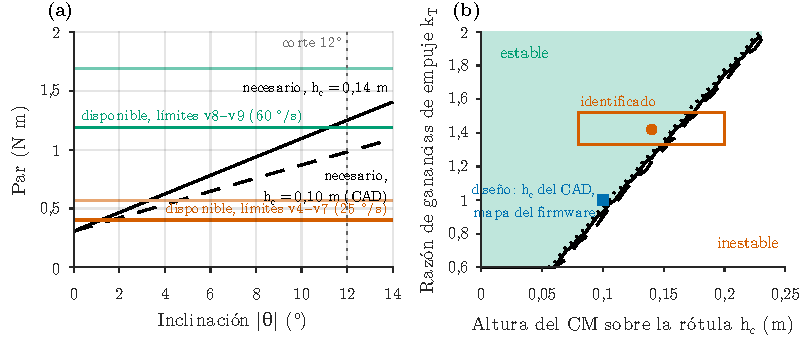
\includegraphics{figures/fig_drone_stability.pdf}
  \caption{Lazo de actitud del octocóptero. (a) Par de gravedad necesario para sostener una inclinación (valores identificado y CAD de $h_c$) y par disponible cuando satura la velocidad angular pedida \eqref{eq:tauavail}, con los límites de banco y de vuelo; líneas gruesas $k_T=1$, líneas finas $k_T=1.42$. (b) Región de estabilidad del modelo lineal completo en el plano $(h_c,k_T)$; la frontera se dibuja para $J=0.12$ (continua), 0,09 (trazos) y \SI{0.15}{\kilo\gram\metre\squared} (puntos). El rectángulo es la incertidumbre identificada y el cuadrado, el punto de diseño ($h_c$ del CAD, mapa del firmware).}
  \label{fig:dronestab}
\end{figure}

\subsubsection{\textit{Ball and plate}}
\label{sec:ballcontrol}

\paragraph{Ley de control}
La ESP32-S3 calcula, para cada eje y para cada cuadro de cámara recibido,
\begin{equation}
  u=u_n+\sat_{\pm220}\Big(k_p\,e+k_i\!\int\!e\,\dd t-k_d\,\hat v\Big),\qquad e=-x_b,
  \label{eq:ballpid}
\end{equation}
con la velocidad $\hat v$ de \eqref{eq:lsvel} que calcula la Pi. El firmware trabaja en unidades de \SI{3}{\milli\metre}; en unidades coherentes con el SI, las ganancias $(1.5;\ 0.8;\ 4.5)$ pasan a $k_p=\SI{0.50}{\micro\second\per\milli\metre}$, $k_i=\SI{0.27}{\micro\second\per\milli\metre\per\second}$ y $k_d=\SI{1.5}{\micro\second\per\milli\metre\second}$. Los pulsos neutros son $u_n=(1386;\ 1392)$\,µs, la integral se limita al 90\% del rango de salida y el juego de la Sección~\ref{sec:linkage} se suma con una rampa de \SI{30}{\micro\second}.

\paragraph{Análisis de estabilidad en tiempo discreto}
Como la derivada actúa a través de un filtro FIR y el lazo contiene varios retardos puros (exposición y transferencia del cuadro, procesamiento, la trama de \SI{50}{\hertz} del servo y el tiempo muerto del servo analógico), el lazo se analizó en tiempo discreto con el periodo de la cámara $h$: la planta \eqref{eq:balltf} con un retraso del servo $\tau_s=\SI{50}{\milli\second}$ se discretizó con retenedor de orden cero, el retardo total $T$ se representó con $T/h$ retardos unitarios, la derivada con el FIR exacto \eqref{eq:lsvel} y la integral con Euler hacia adelante, y la estabilidad se decidió con las raíces del polinomio característico en lazo cerrado. La Fig.~\ref{fig:ballstab}a muestra el mayor $k_d$ estable (en unidades del firmware) en función de $T$ para varias ganancias de planta. Con la ganancia del CAD, $K_b=6.0$, el $k_d=4.5$ nominal solo es estable si $T\lesssim\SI{40}{\milli\second}$, menos que la suma de los retardos del cuadro, del procesamiento, de la trama del servo de \SI{50}{\hertz} y del tiempo muerto del servo. En banco, $k_d=4.5$ fue estable y $k_d=6$ inestable con los rotores apagados; para retardos plausibles ($T=$ 60--\SI{180}{\milli\second}) el modelo reproduce ambas observaciones solo con una ganancia efectiva $K_{b,\mathrm{eff}}=3.5$--4,9 (58--82\% del valor del CAD), donde las ganancias más altas corresponden a los retardos más cortos. La reducción es coherente con el juego del mecanismo, cuya función descriptiva baja la ganancia de pequeña señal, y con una regresión directa de la aceleración de la bola sobre los pulsos de servo registrados, que da 2,5 y 4,9 para los ejes $x$ e $y$ ($R^2=0.29$ y 0,45, limitada por el registro de los pulsos a 20\,Hz). Para $K_{b,\mathrm{eff}}=4.2$ y $T=\SI{0.10}{\second}$ el lazo cerrado tiene un modo rápido poco amortiguado a \SI{1.3}{\hertz} ($\zeta=0.06$), la firma de operar cerca del límite por retardo, y un modo integral lento a \SI{0.064}{\hertz} ($\zeta=0.37$, periodo de \SI{16}{\second}).

\begin{figure}[!htbp]
  \centering
  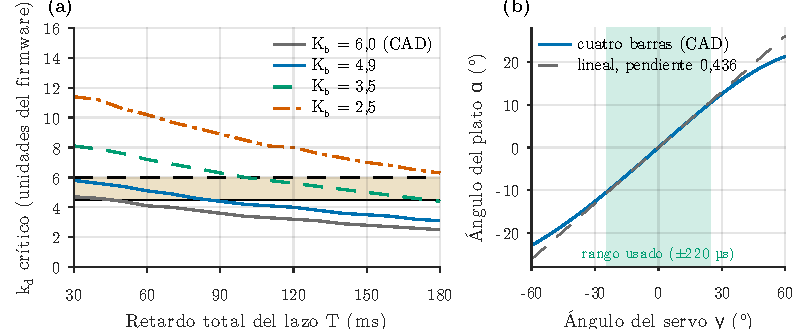
\includegraphics{figures/fig_ball_stability.pdf}
  \caption{\textit{Ball and plate}. (a) Mayor ganancia derivativa estable (unidades del firmware, $k_p=1.5$, $k_i=0.8$) frente al retardo total del lazo para cuatro ganancias de planta; la banda sombreada está acotada por la ganancia que fue estable en banco ($k_d=4.5$, línea continua) y la que no lo fue ($k_d=6$, trazos). (b) Ángulo del plato frente al ángulo del servo según la solución cerrada del cuatro barras \eqref{eq:freud} y su linealización.}
  \label{fig:ballstab}
\end{figure}

\subsubsection{Base móvil}
\label{sec:basecontrol}
Cada rueda tiene un lazo PI de velocidad con integración condicional (la integral se congela cuando la salida satura en 0 o 100\% de ciclo de trabajo), con PWM de \SI{1}{\kilo\hertz}. El modo de ir a un punto usa el error polar $\rho=\|\vect p_g-\vect p\|$, $e_\psi=\operatorname{atan2}(\Delta y,\Delta x)-\psi$, cuya cinemática se sigue de \eqref{eq:diff}: $\dot\rho=-v\cos e_\psi$, $\dot e_\psi=-\omega+(v/\rho)\sin e_\psi$. La ley es $\omega=\sat_{0.2}(1.2e_\psi)$, con $v=0$ mientras $|e_\psi|>\SI{0.2}{\radian}$ y $v=\min\{0.05;\ \max(0.025;\ 0.8\rho)\}$\,m/s en otro caso, y se detiene cuando $\rho<\SI{2}{\centi\metre}$. Como ninguna realimentación suave e invariante en el tiempo puede estabilizar la pose completa de un uniciclo \cite{brockett1983}, la ley solo regula la posición; su convergencia se sigue de cotas elementales. En la fase de giro, $|e_\psi|$ disminuye a no menos de \SI{0.2}{\radian\per\second} hasta que $|e_\psi|\le0.2$. En la fase de avance, $\dot\rho\le-0.025\cos0.2<0$, y $V=e_\psi^2/2$ cumple $\dot V\le-(\omega/e_\psi-v/\rho)\,e_\psi^2$ con $\omega/e_\psi\ge1$ y $v/\rho\le0.8$ para $\rho\ge\SI{3.1}{\centi\metre}$, de modo que $|e_\psi|$ no crece y el robot alcanza la tolerancia en tiempo finito tras a lo sumo una fase de giro.

\subsubsection{Altura y rumbo del octocóptero (firmware v11)}
\label{sec:altura}
\paragraph{Rumbo sobre la base} El octocóptero funciona de forma independiente: no recibe datos de la base. En ralentí ($\le\SI{1400}{\micro\second}$), mientras va montado sobre la base, mantiene el rumbo con que arrancó, pero con una \emph{ventana deslizante} de $\pm\SI{20}{\degree}$. Si un giro de la base lo arrastra más allá, la referencia se desliza con él en lugar de cortar los motores. Así no pelea contra la rótula en un giro de \SI{360}{\degree}, y al detenerse la base queda quieto con un desfase de \SI{20}{\degree} como máximo. Queda un corte de seguridad a \SI{120}{\degree\per\second}. Por encima de \SI{1400}{\micro\second} se conserva el comportamiento de v9: mantener el rumbo con cortes a \SI{20}{\degree} y \SI{35}{\degree\per\second}. Con el v9, los giros de la base terminaban en el corte de \SI{20}{\degree}.

\paragraph{Medición de altura} El VL53L0X no dio ninguna medida válida en los vuelos del 20/11. El \SI{80}{\percent} de las lecturas tuvo el código 2 (\emph{signal fail}): la señal de retorno desde el piso del laboratorio (0,06--\SI{0.3}{MCPS}) quedaba por debajo de la luz ambiente infrarroja (0,7--\SI{0.99}{MCPS}). Se aplicaron cuatro medidas:
\begin{enumerate}[label=(\roman*)]
  \item un \emph{blanco} blanco mate (una hoja A4) fijo en la base bajo el sensor, que multiplica la señal por 2 a 10. Al estar en la base, el láser mide la posición del módulo en la guía, que es la variable que interesa, y no depende del piso ni de la rampa;
  \item el perfil de largo alcance del sensor, con un límite de señal de \SI{0.05}{MCPS}, una sigma de hasta \SI{60}{\milli\metre} y \SI{66}{\milli\second} por medida;
  \item una mediana de tres lecturas con rechazo de saltos de más de \SI{60}{\milli\metre};
  \item una calibración lineal con regla en dos alturas de la guía: $d=0.930\,d_m-\SI{36.5}{\milli\metre}$.
\end{enumerate}
Con eso, las medidas aceptadas pasaron del \SI{0}{\percent} a casi el \SI{100}{\percent}, y la lectura quedó en 317--\SI{334}{\milli\metre} frente a \SI{330}{\milli\metre} medidos con regla.

\paragraph{Corrección por la posición del sensor} El láser está en el brazo 8 ($+x$), a una distancia horizontal $r_s$ del eje de la rótula. Cuando el módulo cabecea un ángulo $\theta$ (positivo con la nariz, $+x$, hacia abajo en la convención FLU) o alabea un ángulo $\phi$, su extremo baja o sube $r_s\sin\theta$, y la distancia medida $d$ cambia aunque la rótula no se mueva por la guía. La altura del eje es
\begin{equation}
  z=d\cos\phi\cos\theta+r_s\sin\theta ,
  \label{eq:brazo}
\end{equation}
que es la que entra al filtro. Con $r_s=\SI{0.20}{\metre}$ (medido), una oscilación de \SI{2}{\degree} en cabeceo aparenta \SI{7}{\milli\metre} de cambio de altura sin la corrección ($0{,}20\sin 2^\circ\approx\SI{7.0}{\milli\metre}$); el firmware aplica \eqref{eq:brazo} a cada medida antes del filtro. Por la misma razón, el acelerómetro de la IMU, también en el brazo 8, mide además las aceleraciones tangencial y centrípeta del giro del módulo ($\dot{\vect\omega}\times\vect r_s+\vect\omega\times(\vect\omega\times\vect r_s)$). A las velocidades angulares del vuelo estacionario, por debajo de \SI{10}{\degree\per\second}, ese término es menor que \SI{0.05}{\metre\per\second\squared} y queda dentro del ruido de proceso del filtro.

\paragraph{Filtro de Kalman de altura} La altura se estima fusionando el láser con el acelerómetro. El estado es $\vect x=[z,\ v,\ b]^{\top}$, con $z$ la distancia al blanco, $v$ la velocidad vertical y $b$ el sesgo del acelerómetro vertical. La predicción se hace a la tasa de la IMU, con la aceleración vertical en el mundo obtenida del acelerómetro filtrado a \SI{10}{\hertz} y de la actitud estimada:
\begin{equation}
  \begin{gathered}
    a_z=\big(-\sin\theta\,a_x+\sin\phi\cos\theta\,a_y+\cos\phi\cos\theta\,a_z^{b}\big)g-g,\\
    z_{k+1}=z_k+v_k\Delta t+\tfrac12(a_z-b_k)\Delta t^2,\quad
    v_{k+1}=v_k+(a_z-b_k)\Delta t,\quad b_{k+1}=b_k .
  \end{gathered}
  \label{eq:kfz}
\end{equation}
El ruido de proceso es $\sigma_a=\SI{0.6}{\metre\per\second\squared}$ sobre la aceleración y $\sigma_b=\SI{0.02}{\metre\per\second\squared}/\sqrt{\mathrm{s}}$ sobre el sesgo. Cada medida aceptada del láser corrige el estado con $R=(\SI{52}{\milli\metre})^2$, que es la dispersión medida sobre el piso. Las correcciones pasan por una puerta de $3\sigma$, y el filtro se resincroniza si rechaza cinco medidas seguidas. En simulación, con el ruido medido, el error de altura baja de \SI{73}{\milli\metre} (láser crudo) a 33--\SI{52}{\milli\metre}. En banco, con el blanco, la incertidumbre del filtro es de unos \SI{23}{\milli\metre}.

\paragraph{Control de altura en cascada} La planta vertical es un doble integrador. Tiene además el retardo del motor (\SI{70}{\milli\second}), el del sensor (\SI{66}{\milli\second} más la mediana) y la fricción seca de la guía, que la hace pegarse y saltar. Por eso un PID sobre la altura oscila. Se usa una cascada:
\begin{equation}
  \begin{gathered}
    v_{\mathrm{ref}}=\mathrm{sat}_{\pm\SI{40}{\milli\metre\per\second}}\!\big(k_z(z_{\mathrm{ref}}-\hat z)\big),\\
    \Delta u=\mathrm{sat}_{\pm\SI{60}{\micro\second}}\!\Big(k_{vp}(v_{\mathrm{ref}}-\hat v)+k_{vi}\!\int(v_{\mathrm{ref}}-\hat v)\,dt\Big),
  \end{gathered}
  \label{eq:cascada}
\end{equation}
con $k_z=\SI{1.5}{\per\second}$, $k_{vp}=\SI{0.18}{\micro\second\per(\milli\metre\per\second)}$, $k_{vi}=\SI{0.35}{\micro\second\per\milli\metre}$ y anti-\emph{windup} en el integrador. La referencia $z_{\mathrm{ref}}$ sigue al objetivo con una rampa de \SI{20}{\milli\metre\per\second}; las órdenes \emph{Subir} y \emph{Bajar} lo mueven en $\pm\SI{20}{\milli\metre}$. El lazo interno usa la velocidad del filtro de Kalman, que llega sin el retraso de derivar la medida del láser, así que frena antes de llegar. Su integrador compensa la caída de tensión de la batería y la fricción.

En simulación, con fricción de Coulomb y adherencia en la guía, la oscilación pico a pico pasa de 13--\SI{46}{\milli\metre} con el PID a 4--\SI{12}{\milli\metre} con la cascada. El modo se activa con \emph{Mantener} solo si la incertidumbre del filtro es menor que \SI{30}{\milli\metre}; si no, se fija el colectivo. La validación en vuelo queda pendiente.

\subsection{Modelo acoplado y propagación de perturbaciones}
\label{sec:coupling}

Combinando el octocóptero linealizado \eqref{eq:pitchlin} cerrado con \eqref{eq:cascade} y la bola \eqref{eq:balllinx} cerrada con \eqref{eq:ballpid} se obtiene la propagación de una aceleración de la base hasta la bola,
\begin{gather}
  X_b(s)=\frac{S_b(s)}{s^2}\Big\{\gamma_b\Big[\big(g-(h_P+\kappa)s^2\big)\,T_{\theta A}(s)-1\Big]A_{J,x}(s)+D_b(s)\Big\}, \label{eq:propag}\\
  T_{\theta A}(s)=\frac{-m h_c\,P(s)}{1+L_D(s)}, \notag
\end{gather}
donde $P(s)=1/(J_ys^2-mgh_c)$, $L_D$ es la función de transferencia en lazo abierto de la cascada de actitud, $S_b=1/(1+L_b)$ es la sensibilidad del lazo de la bola y $D_b$ reúne todas las perturbaciones que actúan directamente sobre la bola (flujo de aire, vibración, juego). La Fig.~\ref{fig:transm} evalúa \eqref{eq:propag}. Destacan tres resultados.

\begin{enumerate}[label=(\roman*)]
  \item \textbf{La rotación y la pendiente son benignas.} La aceleración centrípeta de la rótula en los giros de la guía (velocidades de rueda de hasta \SI{0.10}{\metre\per\second}) es como mucho \SI{0.024}{\metre\per\second\squared} alrededor del punto medio del eje y \SI{0.015}{\metre\per\second\squared} alrededor de una rueda, equivalente a una inclinación del plato menor que \SI{0.15}{\degree}; la pendiente no entra en absoluto en la ecuación de la bola \eqref{eq:tilt}. Solo las transiciones de la rampa y el arranque y la parada de la base producen aceleraciones significativas.
  \item \textbf{El octocóptero amplifica las aceleraciones lentas de la base.} Como su rigidez neta \eqref{eq:stiff} es pequeña, el módulo responde a las aceleraciones de la base cercanas a su modo lento (0,2--\SI{0.3}{\hertz}) con inclinaciones de varios grados por m/s$^2$ (Fig.~\ref{fig:transm}b), y entre 0,1 y \SI{1}{\hertz} este camino domina sobre el camino directo a la bola (Fig.~\ref{fig:transm}c). Esto es coherente con los cortes por inclinación en los bordes de la rampa en las pruebas integradas. Es el costo dinámico del dron frente a un cardán rígido (Sección~\ref{sec:porquedron}).
  \item \textbf{El movimiento de actitud no es la fuente principal del error de la bola.} Al filtrar la actitud medida del octocóptero en ralentí (registro de banco, RMS 0,23--\SI{0.37}{\degree}) por $X_b/\Theta$ se predice un RMS de la bola de solo 1,7--\SI{2.1}{\milli\metre}, mientras que el RMS medido con los rotores girando y la base quieta es 16--\SI{21}{\milli\metre} en $x$ y 10--\SI{12}{\milli\metre} en $y$. Más del 90\% de la varianza medida está por debajo de \SI{0.3}{\hertz}, con picos espectrales entre 0,02 y \SI{0.05}{\hertz} (periodos de 20--45\,s), la escala de tiempo del modo integral lento del lazo de la bola (\SI{0.064}{\hertz}). La perturbación dominante es, por tanto, una carga lentamente variable que actúa directamente sobre la bola ($D_b$): el flujo de los rotores sobre el plato, la deriva inducida por la vibración y el juego, que llevaban la bola hacia $(-x,-y)$ en las pruebas. Solo la rechaza la acción integral, cuyo ancho de banda limita el retardo.
\end{enumerate}

\begin{figure}[!htbp]
  \centering
  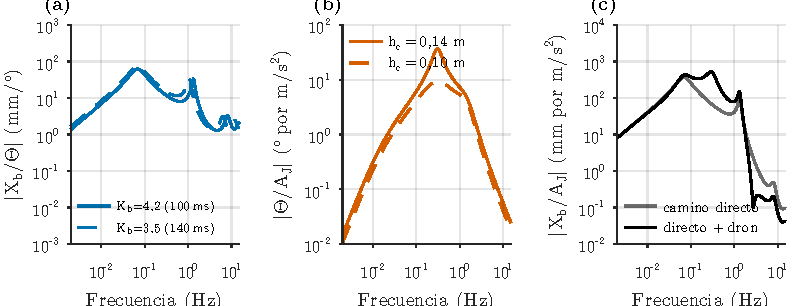
\includegraphics{figures/fig_transmissibility.pdf}
  \caption{Propagación de perturbaciones predicha por \eqref{eq:propag} (ganancias de vuelo estacionario, $k_T=1.42$). (a) Desplazamiento de la bola por grado de inclinación del octocóptero con el lazo de la bola cerrado. (b) Inclinación del octocóptero por unidad de aceleración de la base. (c) Desplazamiento de la bola por unidad de aceleración de la base, por el camino directo y a través del octocóptero.}
  \label{fig:transm}
\end{figure}

\subsection{Limitaciones fundamentales e implicaciones de diseño}
\label{sec:limits_fund}
El modelo también acota lo que cualquier controlador puede lograr con el hardware actual \cite{skogestad2005}.
\begin{itemize}
  \item \textbf{Octocóptero.} Un polo inestable $p$ exige un cruce por encima de $\approx2p$, y un retardo efectivo $\theta_e$ lo limita a $\approx1/\theta_e$; la estabilización robusta requiere aproximadamente $p\,\theta_e<0.5$. Con $p=\SI{6.1}{\radian\per\second}$ y $\theta_e\approx\tau_m+T_a=\SI{0.09}{\second}$, $p\theta_e=0.55$: el control de actitud del módulo en la rótula opera en el borde de este límite. El remedio estructural es bajar el centro de masa: con las baterías bajo la rótula ($h_c<0$) el módulo se vuelve un péndulo estable y la autoridad que exige \eqref{eq:thetastar} disminuye; además, las baterías bajas mejorarían el vuelco en la rampa.
  \item \textbf{\textit{Ball and plate}.} El cero en el semiplano derecho $z_1=\SI{15.2}{\radian\per\second}$ limita el cruce a $\approx z_1/2=\SI{7.6}{\radian\per\second}$, y el retardo de $\approx$\SI{0.1}{\second}, a $\approx\SI{10}{\radian\per\second}$; el PID opera en $K_{b,\mathrm{eff}}k_d\approx\SI{6}{\radian\per\second}$, cerca de ambas cotas, lo que explica el techo de $k_d$. Un control más rápido de la bola exige un retardo menor (servos digitales a \SI{333}{\hertz}, actualización de los servos sincronizada con los cuadros) y un $\kappa$ menor (la superficie del plato más cerca del centro de la junta universal).
  \item \textbf{Base.} El margen de aceleración \eqref{eq:tip} y el modo lento del octocóptero piden referencias suaves (con jerk limitado) para la base; en una pendiente de \SI{20}{\degree} el margen de aceleración sin empuje es de solo \SI{0.26}{\metre\per\second\squared}; con los rotores sosteniendo el 35--55\% del peso del módulo sube a 0,7--\SI{1.0}{\metre\per\second\squared} (Sección~\ref{sec:porquedron}). Las alternativas son un lastre bajo o un módulo aéreo más bajo.
  \item \textbf{Energía.} El margen de empuje cae con el cuadrado de la tensión de la batería (Sección~\ref{sec:bateria}); sin medición de tensión y compensación del colectivo, el tiempo útil de vuelo es de 3--\SI{7}{\minute} por par de LiPo.
\end{itemize}
